\begin{frame}
  \frametitle{センサーボードを使う}
  \begin{itemize}
    \item 複数のセンサーを使ったプログラム
    \item LEDを使ったプログラムの復習
    \item ボタンとLEDを使ったプログラム
  \end{itemize}
\end{frame}

\begin{frame}
  \frametitle{センサーボードってなんだろう}
  \begin{columns}
    \begin{column}{0.48\textwidth}
      \begin{itemize}
        \item 4色のLED
        \item 照度センサー
        \item 赤外線LED
        \item 赤外線受信ユニット
        \item 温湿度気圧センサー
      \end{itemize}
    \end{column}
    \begin{column}{0.48\textwidth}
      \begin{figure}
        \centering

        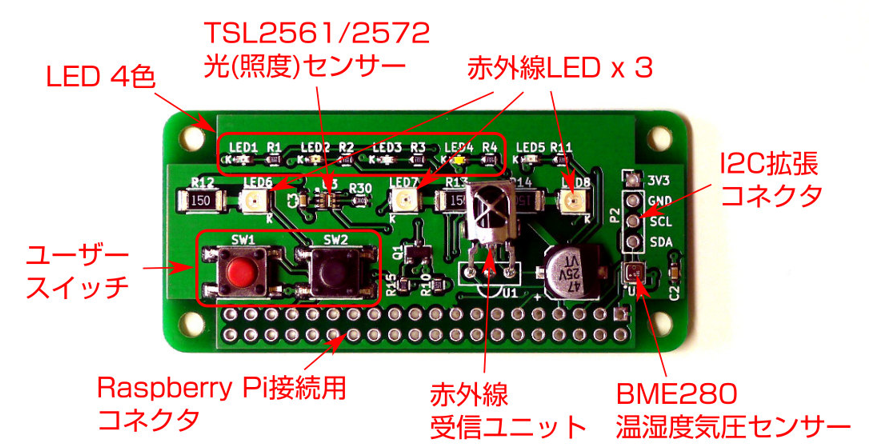
\includegraphics[width=1.0\textwidth]{../images/chap03/sensors_name.png}
        \caption{センサーボード}
      \end{figure}
    \end{column}
  \end{columns}
\end{frame}

\begin{frame}
  \frametitle{センサーボードを取り付けよう}
  \begin{figure}
    \centering
    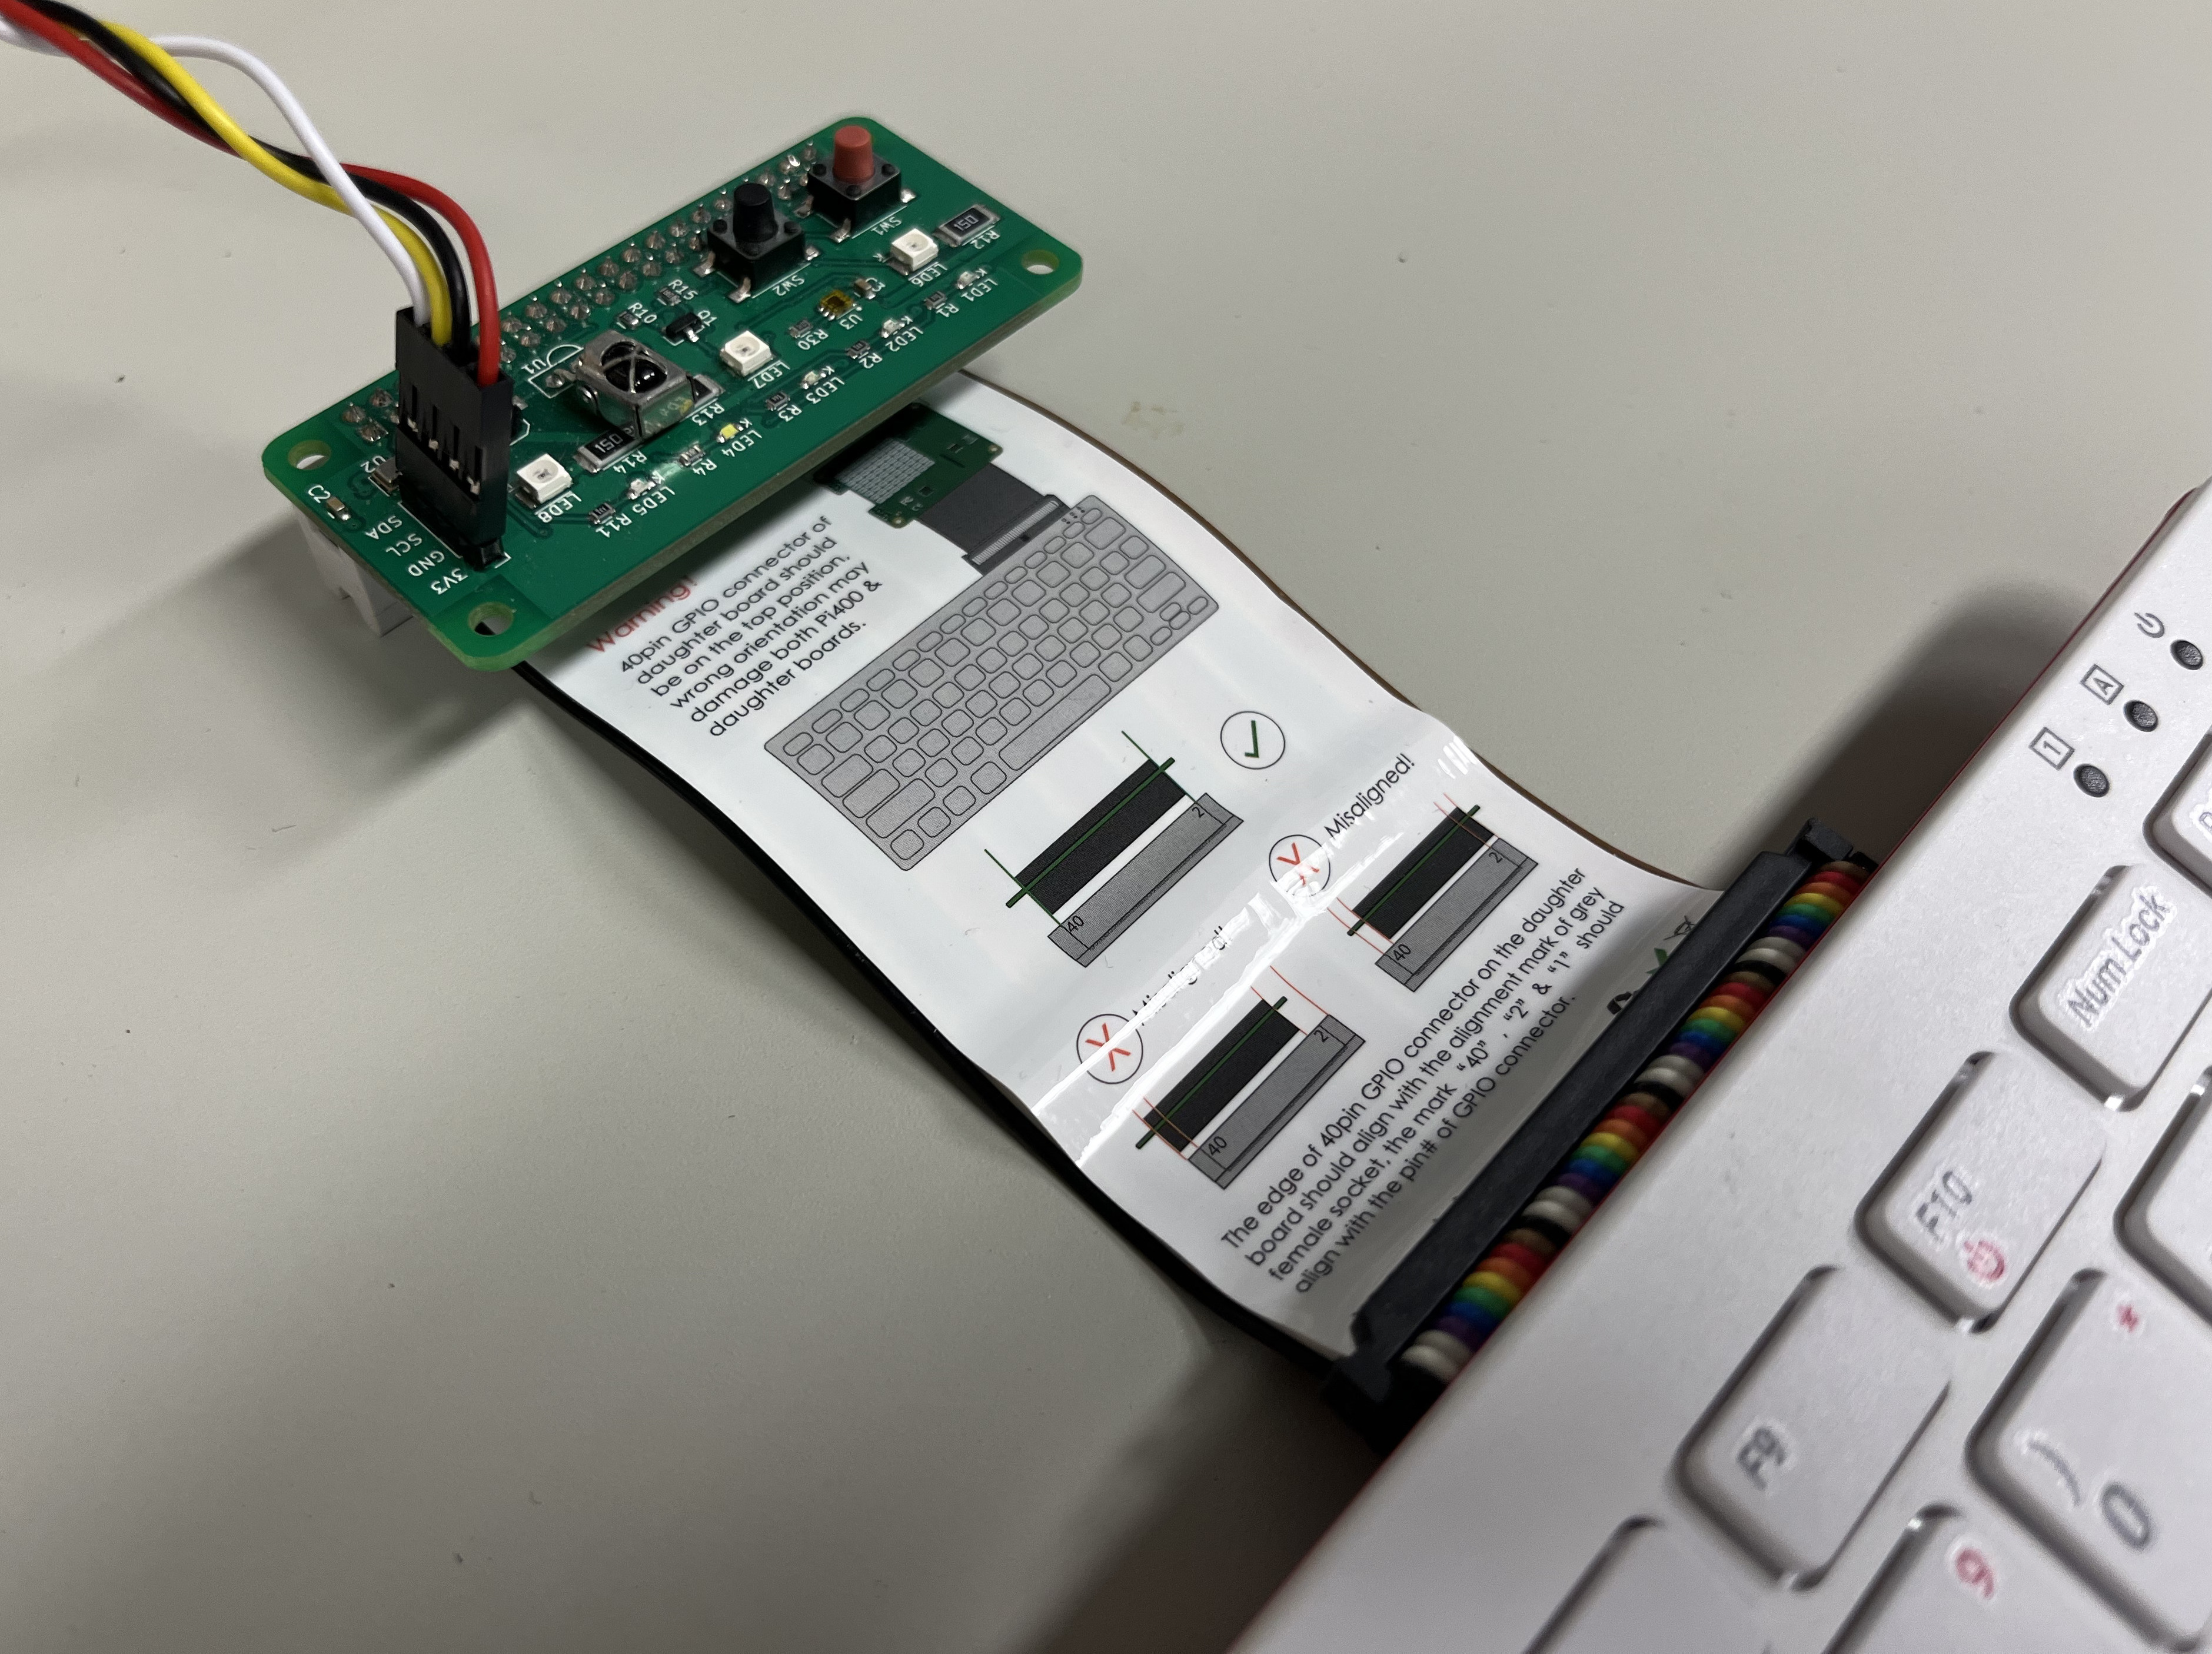
\includegraphics[width=0.5\textwidth]{../images/chap03/how_to_install_bme280.jpg}
    \caption{外付けのセンサー}
  \end{figure}
  \begin{itemize}
    \item 一度シャットダウンしてからセンサーボードを差し込む
    \item 赤色の線が3V3に来るようにする
  \end{itemize}
\end{frame}

\begin{frame}
  \frametitle{センサーボードとラズパイの関係}
  \begin{figure}
%    \centering
%    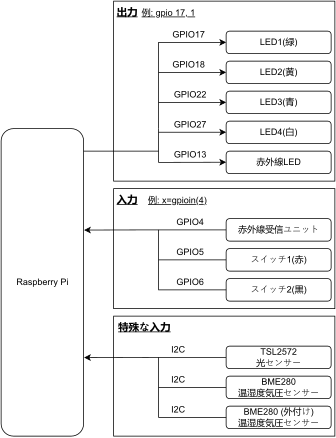
\includegraphics[height=0.9\textheight]{../images/chap03/rpz-ir-sensor.svg}
    \includesvg[height=0.9\textheight]{../images/chap03/rpz-ir-sensor.svg}
\end{figure}
\end{frame}


% \begin{frame}
%   \frametitle{LEDを光らせてみよう(1)}
%   \begin{itemize}
%     \item led.hspを実行しよう
%           \begin{itemize}
%             \item 03ディレクトリに移動しよう
%             \item ターミナルで hsed コマンドを使おう
%             \item ファイル\rightarrow 開く\rightarrow led.hsp
%           \end{itemize}
%   \end{itemize}
% \end{frame}

% \begin{frame}[fragile]
%   \frametitle{LEDを光らせてみよう(2)}
%   \begin{lstlisting}[title=led.hsp,label=led.hsp]
%   #include "hsp3dish.as"   <#blue#; スクリプトの設定を読み込む#>
%   #include "rpz-gpio.as"   <#blue#; スクリプトの設定を読み込む#>
%           redraw 0         <#blue#; 画面更新 (仮想画面に描画)#>
%           font "",30       <#blue#;文字のフォント、サイズを決める#>
%           pos 20, 20       <#blue#;文字の場所を決める#>
%           mes "LEDが光るよ" <#blue#;文字を決める#>
%           redraw 1         <#blue#;画面更新(実際の画面に描画)#>
%   *led
%           gpio 17, 1     <#blue#;GPIO17を点灯させる#>
%           wait 100       <#blue#;0.1 秒待つ#>
%           goto *led      <#blue#;*led まで戻る#>
%           gpio 17, 0     <#blue#;GPIO17を消灯させる#>
%   \end{lstlisting}
% \end{frame}

% \begin{frame}
%   \frametitle{LEDを光らせてみよう(3)}
%   \begin{itemize}
%     \item gpio 17, 1 の部分でLEDを光らせているよ
%           \begin{itemize}
%             \item 17 は光らせたいLEDのGPIO番号
%             \item 1で点灯、0で消灯
%           \end{itemize}
%   \end{itemize}
% \end{frame}

% \begin{frame}
%   \frametitle{問題をといてみよう!}
%   \begin{itemize}
%     \item 教科書28ページ 問題3-7(4問)
%   \end{itemize}
% \end{frame}


\begin{frame}[fragile]
  \frametitle{温湿度/気圧/明るさを調べる-1}
  \begin{lstlisting}[title=\sim/03/sensors.hsp 前半, label=sensors.hsp-1]
   #include "hsp3dish.as"    
   #include "jtalk.as"    

   init_bme               <#blue#; 温湿度気圧センサ#>
   if stat {              <#blue#; 初期化成功チェック#>
     redraw 0          
     mes "failed to init bme: " + stat
     redraw 1
     stop
   }

   geti2c_lux_init     <#blue#; 照度センサ tsl2572 を初期化する#>

   *main
   redraw 0            <#blue#; 仮想画面に描画#>
   pos 60, 60          <#blue#; 表示位置を設定#>
  
  \end{lstlisting}
\end{frame}

\begin{frame}[fragile]
  \frametitle{温湿度/気圧/明るさを調べる-2}
  \begin{lstlisting}[title=\sim/03/sensors.hsp 後半, label=sensors.hsp-2]
  get_humidity          <#blue#; rpz_humに湿度取得#>
  hum = rpz_hum       
  get_pressure          <#blue#; rpz_pressに気圧取得#>
  press = rpz_press
  geti2_lux_als         <#blue#; rpz_luxに照度取得#>
  lux = rpz_lux
  mes "温度: " + temp + " [℃]" <#blue#; 取得したデータの表示#>
  mes "湿度: " + hum + " [%]"
  mes "気圧: " + press + "[hPa]"
  mes "照度: " + lux + " [lx]"
  redraw 1              
  wait 100
  goto *main
  \end{lstlisting}
\end{frame}

\begin{frame}
  \begin{exampleblock}{問題をといてみよう!}
    \begin{itemize}
      \item \sim/03/sensors.hspを実行しよう
      \item 教科書23ページ 問題3-6(8問)
    \end{itemize}
  \end{exampleblock} 
\end{frame}


\begin{frame}[fragile]
  \frametitle{LEDをチカチカさせよう}
  \begin{lstlisting}[title=\sim/03/Ltika.hsp,label=Ltika.hsp]
    #include "hsp3dish.as"		<#blue#;スクリプトの設定を読み込む#>
    #include "rpz-gpio.as"		<#blue#;スクリプトの設定を読み込む#>
      redraw 0		<#blue#;画面更新(仮想画面に描画)#>
      mes "0.5 秒毎に青色の LED がチカチカするよ"
      redraw 1		<#blue#;画面更新(実際の画面に描画)#>
    *led
      gpio 22,0		<#blue#;gpio22 を消灯#>
      wait 50 		<#blue#;500 ミリ秒待つ#>
      gpio 22, 1 		<#blue#;gpio22 を点灯#>
      wait 50 		<#blue#;500 ミリ秒待つ#>
      goto *led 		<#blue#;*led にジャンプ(繰り返し)#>
  \end{lstlisting}
\end{frame}

\begin{frame}
  \begin{exampleblock}{問題をといてみよう!}
    \begin{itemize}
      \item \sim/03/Ltika.hspを実行しよう
      \item 教科書25ページ 問題3-7(6問)
    \end{itemize}
  \end{exampleblock} 
\end{frame}

\begin{frame}[fragile]
  \frametitle{ボタンを使ってLEDをつけてみよう}
  \begin{lstlisting}[title=\sim/03/button\_led.hsp, label=button_led.hsp]
  #include "hsp3dish.as"
  #include "rpz-gpio.as"
  
          gpio 17, 0
          gpio 18, 0
          gpio 22, 0
          gpio 27, 0

          redraw 0
          font "", 30
          pos 20, 20
          mes "ボタンを押している間 LED が光るよ"
          redraw 1
  *led
          bnt1 = gpioin(5)        <#blue#;ボタンの状態を調べる#>
          if btn1=0 : gpio 18, 1  <#blue#;ボタンによってLEDを点灯/消灯#>
          wait 10                 <#blue#;0.1秒待つ#>
          goto *led               <#blue#;*ledに戻る#>
  \end{lstlisting}
\end{frame}

\begin{frame}
  \frametitle{ボタンが押されているか調べる命令}
  \begin{itemize}
    \item gpioin()
          \begin{itemize}
            \item ()の中にはGPIO番号が入るよ
            \item 赤ボタンならGPIO=5、黒ボタンならGPIO=6
          \end{itemize}
    \item ima\_btn = gpioin(5)
          \begin{itemize}
            \item GPIO5(赤ボタン)が押されたかどうかを数字で判定
            \item 押されたらima\_btn=0、はなされたらima\_btn=1
          \end{itemize}
  \end{itemize}
\end{frame}

\begin{frame}
  \begin{exampleblock}{問題をといてみよう!}
    \begin{itemize}
      \item \sim/03/button\_led.hspを実行しよう
      \item 教科書27ページ 問題3-8(4問)
    \end{itemize}
  \end{exampleblock} 
\end{frame}

\begin{frame}[fragile]
  \frametitle{ボタンを使ってLEDをつけてみよう(2)-1}
  \begin{lstlisting}[title=\sim/03/button\_led2.hsp 前半, label=button_led2.hsp-1]
  #include "hsp3dish.as"
  #include "rpz-gpio.as"
  
          gpio 17, 0
          gpio 18, 0
          gpio 22, 0
          gpio 27, 0
        
          redraw 0
          font "", 30
          pos 20, 20
          mes "赤いボタンを押して、LED をつけたり消したりできるよ"
          redraw 1

          ima_btn = 1   <#blue#;今ボタンを押しているかどうかの変数#>
          mae_btn = 1   <#blue#;前回はボタンを押しているかどうかの変数#>
          led = 1       <#blue#;LEDを光らせるか決める変数#>
  \end{lstlisting}
\end{frame}

\begin{frame}[fragile]
  \frametitle{ボタンを使ってLEDをつけてみよう(2)-2}
  \begin{lstlisting}[title=\sim/03/button\_led2.hsp 後半, label=button_led2.hsp-2]
  *hata
          ima_btn = gpioin(5)
          if ima_btn = 0{    <#blue#;今押されているとき#>
            if mae_btn = 1{  <#blue#;前は押されていなかった時#>
              led = 1 - led  <#blue#;LEDの消灯を切り替える#>
            }
          }

          gpio 22, led       <#blue#;GPIO22をつけるか消すかする#>
          mae_btn = ima_btn  <#blue#;今の状態を前回の状態とする#>

          wait 10
          goto *hata
  \end{lstlisting}
\end{frame}

\begin{frame}
  \frametitle{ボタンを押してLEDをon/offするには}
  \begin{itemize}
    \item ボタンを押したかどうやってわかるの?
  \end{itemize}
  \begin{figure}
    \centering
    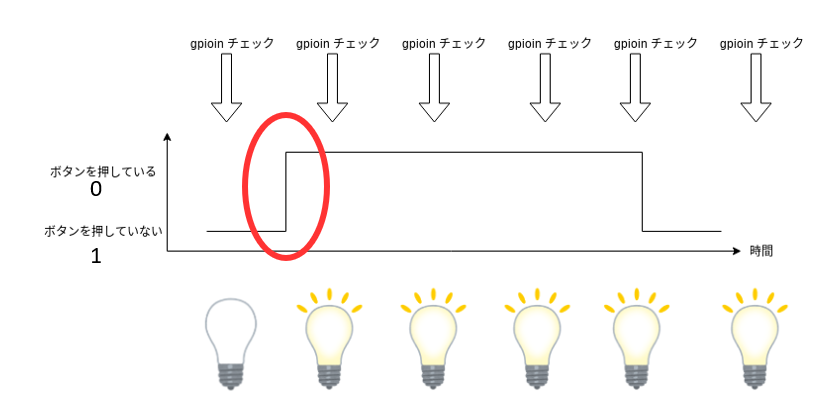
\includegraphics[width=0.6\textwidth]{../images/chap03/button_push.png}
  \end{figure}
  \begin{itemize}
    \item 赤い部分は押されていない状態から押されている状態に変化($1\rightarrow0$)したことを示す
    \item 変化したことをラズベリーパイが確認し、LEDの状態を変化させる
  \end{itemize}
\end{frame}

\begin{frame}
  \begin{exampleblock}{問題をといてみよう!}
    \begin{itemize}
      \item \sim/03/button\_led2.hspを実行しよう
      \item 教科書30ページ 問題3-9(3問)
    \end{itemize}
  \end{exampleblock} 
\end{frame}

\begin{frame}[fragile]
  \frametitle{ボタンを使って光るLEDを変えてみよう-1}
  \begin{lstlisting}[title=\sim/03/button\_led3.hsp 前半, label=button_led3.hsp-1]
  #include "hsp3dish.as"
  #include "rpz-gpio.as"
  
          gpio 17, 0   
          gpio 18, 0
          gpio 22, 0
          gpio 27, 0

          redraw 0
          font "", 30
          pos 20, 20
          mes "赤いボタンを押して、LED をつけたり消したりできるよ"
          redraw 1

          ima_btn = 1 
          ledidx = 0  <#blue#;ledidxを初期化#>
  \end{lstlisting}
\end{frame}

\begin{frame}[fragile]
  \frametitle{ボタンを使って光るLEDを変えてみよう-2}
  \begin{lstlisting}[title=\sim/03/button\_led3.hsp 中盤, label=button_led3.hsp-2]
  *hata
          ima_btn = gpioin(5)
          if ima_btn = 0{           <#blue#;今押されているとき#>
           iedidx = (ledidx+1) \ 4  <#blue#;ledidxで何番目のLEDを光らせるか決める#>
           if ledidx=1 {            <#blue#;1番目の時はGPIO17のLEDを光らせる#>
             gpio 17, 1             <#blue#;(0+1)\4 = 1#>
             gpio 18, 0 
             gpio 22, 0
             gpio 27, 0
           }

           else : if ledidx=2 {     <#blue#;2番目の時はGPIO18のLEDを光らせる#>
             gpio 17, 0             <#blue#;(1+1)\4 = 2#>
             gpio 18, 1
             gpio 22, 0
             gpio 27, 0
           }
  \end{lstlisting}
\end{frame}

\begin{frame}[fragile]
  \frametitle{ボタンを使って光るLEDを変えてみよう-3}
  \begin{lstlisting}[title=button\_led3.hsp 後半, label=button_led3.hsp-3]
           else : if ledidx=3{      <#blue#;3番目の時はGPIO22のLEDを光らせる#>
             gpio 17, 0             <#blue#;(2+1)\4 = 3#>
             gpio 18, 0
             gpio 22, 1
             gpio 27, 0
           }

           else : if ledidx=0 {     <#blue#;4番目の時はGPIO27のLEDを光らせる#>
             gpio 17, 0             <#blue#;(3+1)\4 = 0#>
             gpio 18, 0
             gpio 22, 0
             gpio 27, 1
           }
          }

          wait 10
          goto *hata
  \end{lstlisting}
\end{frame}

\begin{frame}
  \frametitle{LEDはどうして動いて見えている?}
  \begin{itemize}
    \item ima\_btn ボタンを押したかどうか調べる
    \item ledidx ボタンを押した回数を調べる
    \begin{itemize}
      \item ledidx = 0のときledidx = $(0+1)\backslash4$
      \begin{itemize}
        \item 計算すると$1\div4$ = 0あまり1なので次のledidx = 1になる
      \end{itemize}
      \item ledidx = 1のときledidx = $(1+1)\backslash4$ 
      \begin{itemize}
        \item 計算すると$2\div4$ = 0あまり2なので次のledidx = 2になる 
      \end{itemize}
      \item ledidx = 2のときledidx = $(2+1)\backslash4$ 
      \begin{itemize}
        \item 計算すると$3\div4$ = 0あまり3なので次のledidx = 3になる
      \end{itemize}
      \item ledidx = 3のときledidx = $(3+1)\backslash4$ 
      \begin{itemize}
        \item 計算すると$4\div4$ = 1あまり0なので次のledidx = 0になる
      \end{itemize}
    \end{itemize}
  \end{itemize}
\end{frame}

\begin{frame}
  \begin{exampleblock}{問題をといてみよう!}
    \begin{itemize}
      \item \sim/03/button\_led3.hspを実行しよう
      \item 教科書32ページ 問題3-10(3問)
    \end{itemize}
  \end{exampleblock} 
\end{frame}
